\documentclass[french,c,
% PDF settings
hyperref={%
    pdftitle={Rappels COVID-19},%
    pdfauthor={Guillaume MULLER},%
    pdfsubject={COVID-19},%
    pdfkeywords={COVID-19}%
    colorlinks=true,%
    urlcolor=blue,%
    linkcolor=%
  },%
xcolor={pdftex,svgnames}, % dvipsnames, dvipsnames*, svgnames, svgnames*, x11names,
]{beamer}  %
\usetheme{Copenhagen}

% Remove navigation bar
\setbeamertemplate{navigation symbols}{}
% Remove outline at top
\setbeamertemplate{headline}{}

% from links
\usepackage{hyperref}

% Correct French/English indentation and splitting of words
\usepackage{babel}

% Correct management of accentuated chars in input file
\usepackage[utf8]{inputenc}
%\usepackage[utf8]{inputenc}

% Correct font for the generation of docs with accentuated chars
\usepackage[T1]{fontenc}      % Can handle hyphenation of words with accented characters

% Insertion of images generated by external tools
\usepackage{graphicx}

% For graphics
\usepackage{tikz}
\usetikzlibrary{calc}


\def\slider#1#2{% 1: length, 2: position of the mark (0 to 1)
  \shorthandoff{:!} % protection in french babel mode
  \tikz[baseline=0cm]{
    \coordinate (start) at (0,0);
    \coordinate (end) at (#1,0);
    \coordinate (mark) at ($(start)!#2!(end)$);
    \fill[left color=blue, right color=red, fill, shading angle=95, rounded corners] (start)[above=.7em] rectangle (end)[below=.7em] ;
    \path[
        fill=blue!30!cyan,
    ] (mark) + (-.3em, -.2em) -- +(0em, -.4em) -- +(.3em, -.2em) -- +(.3em, .9em) -- +(-.3em, .9em) -- cycle;
  }
  \shorthandon{:!}
}

%%%%%%%%%%%%%%%%%%%%%%%%%%%%%%%%%%%%%%%%%%%%%%%%%%%%%%%%%%%%%%%%%%%%%%
\begin{document}


%%%%%%%%%%%%%%%%%%%%%%%%%%%%%%%%%%%%%%%%
% First slide
\begin{frame}{Rappels COVID-19}

  \onslide<1>{ \hspace{4cm} \raisebox{-.45\height}{
\includegraphics[width=3em]{images/dont-panic.png}}}

  \begin{itemize}
    \item[] \raisebox{-.45\height}{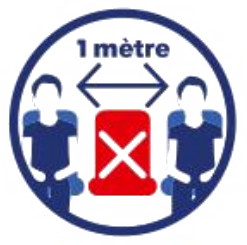
\includegraphics[width=2.5em]{images/distance.png}} \hspace{.3cm}
      Garder les \textbf{distances} { \scriptsize ($>$1~m) }
    \item[] \raisebox{-.45\height}{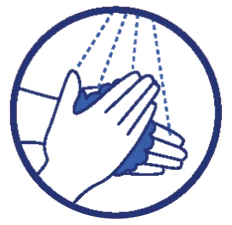
\includegraphics[width=2.5em]{images/lavage_mains.png}} \hspace{.3cm}
      Se laver régulièrement les \textbf{mains} { \scriptsize ($\approx$30 min.) }
    \item[] \raisebox{-.45\height}{
\includegraphics[width=2.5em]{images/masque.png}} \hspace{.3cm}
      Mettre un \textbf{masque} { \scriptsize (intérieur+dense, \textbf{nez}+bouche) }
    \item[] \raisebox{-.45\height}{
\includegraphics[width=2.5em]{images/windows10.png}} \hspace{.3cm}
      Ouvrir les \textbf{fenêtres} régulièrement { \scriptsize ($\approx$3 hr.)}
  \end{itemize}

  \begin{center}
    \onslide*<2>{ \bigskip COOL \slider{10em}{0.7} PARANO }
    \onslide*<3>{ 
\includegraphics[width=10em]{images/raising-hands.png} }
  \end{center}

\end{frame}

\end{document}


%%% Local Variables:
%%% mode: latex
%%% TeX-master: t
%%% End:
